% % % % % % % % % % % % % % % % % % % % % % % % % % % % % % % % % % % % % % % %
% IEEE Style - Double columns, 11pt font, letterpaper
\documentclass[journal, twocolumn, final,11pt,letterpaper]{IEEEtran}	

% Include Latex Packages
\usepackage{etex}	% This package enables the use of many packages

% % Page styles
\usepackage{setspace}	% line spacing package
\doublespacing			% use double spacing
%\linespread{1.6}		% Use linespread to fine tune line spacing, not recommended


% % Figures
\usepackage{float}		% improves interface for floating objects
\usepackage{subfig}		% enables subfloat
\usepackage{graphicx}	% more image type support
\usepackage{circuitikz}
\usepackage{epstopdf}	% automatically convert included eps files to pdf
\usepackage{tikz}
%\usepackage{listings}
\usepackage{color}
\definecolor{dkgreen}{rgb}{0,0.6,0}
\definecolor{gray}{rgb}{0.5,0.5,0.5}
\definecolor{mauve}{rgb}{0.58,0,0.82}

\lstset{frame=tb,
	language=Verilog,
	aboveskip=3mm,
	belowskip=3mm,
	showstringspaces=false,
	columns=flexible,
	basicstyle={\small\ttfamily},
	numbers=none,
	numberstyle=\tiny\color{gray},
	keywordstyle=\color{blue},
	commentstyle=\color{dkgreen},
	stringstyle=\color{mauve},
	breaklines=true,
	breakatwhitespace=true,
	tabsize=3
}
\usetikzlibrary{matrix,calc}
\usetikzlibrary{shapes}

\newcommand*{\circled}[2][red]{
	\tikz[baseline=(char.base)]{
		\node[shape=ellipse,inner sep=1pt,
		draw=#1,
		] (char) {#2};}
}

%isolated term
%#1 - Optional. Space between node and grouping line. Default=0
%#2 - node
%#3 - filling color
\newcommand{\implicantsol}[3][0]{
	\draw[rounded corners=3pt, fill=#3, opacity=0.3] ($(#2.north west)+(135:#1)$) rectangle ($(#2.south east)+(-45:#1)$);
}


%internal group
%#1 - Optional. Space between node and grouping line. Default=0
%#2 - top left node
%#3 - bottom right node
%#4 - filling color
\newcommand{\implicant}[4][0]{
	\draw[rounded corners=3pt, fill=#4, opacity=0.3] ($(#2.north west)+(135:#1)$) rectangle ($(#3.south east)+(-45:#1)$);
}

%group lateral borders
%#1 - Optional. Space between node and grouping line. Default=0
%#2 - top left node
%#3 - bottom right node
%#4 - filling color
\newcommand{\implicantcostats}[4][0]{
	\draw[rounded corners=3pt, fill=#4, opacity=0.3] ($(rf.east |- #2.north)+(90:#1)$)-| ($(#2.east)+(0:#1)$) |- ($(rf.east |- #3.south)+(-90:#1)$);
	\draw[rounded corners=3pt, fill=#4, opacity=0.3] ($(cf.west |- #2.north)+(90:#1)$) -| ($(#3.west)+(180:#1)$) |- ($(cf.west |- #3.south)+(-90:#1)$);
}

%group top-bottom borders
%#1 - Optional. Space between node and grouping line. Default=0
%#2 - top left node
%#3 - bottom right node
%#4 - filling color
\newcommand{\implicantdaltbaix}[4][0]{
	\draw[rounded corners=3pt, fill=#4, opacity=0.3] ($(cf.south -| #2.west)+(180:#1)$) |- ($(#2.south)+(-90:#1)$) -| ($(cf.south -| #3.east)+(0:#1)$);
	\draw[rounded corners=3pt, fill=#4, opacity=0.3] ($(rf.north -| #2.west)+(180:#1)$) |- ($(#3.north)+(90:#1)$) -| ($(rf.north -| #3.east)+(0:#1)$);
}

%group corners
%#1 - Optional. Space between node and grouping line. Default=0
%#2 - filling color
\newcommand{\implicantcantons}[2][0]{
	\draw[rounded corners=3pt, opacity=.3] ($(rf.east |- 0.south)+(-90:#1)$) -| ($(0.east |- cf.south)+(0:#1)$);
	\draw[rounded corners=3pt, opacity=.3] ($(rf.east |- 8.north)+(90:#1)$) -| ($(8.east |- rf.north)+(0:#1)$);
	\draw[rounded corners=3pt, opacity=.3] ($(cf.west |- 2.south)+(-90:#1)$) -| ($(2.west |- cf.south)+(180:#1)$);
	\draw[rounded corners=3pt, opacity=.3] ($(cf.west |- 10.north)+(90:#1)$) -| ($(10.west |- rf.north)+(180:#1)$);
	\fill[rounded corners=3pt, fill=#2, opacity=.3] ($(rf.east |- 0.south)+(-90:#1)$) -|  ($(0.east |- cf.south)+(0:#1)$) [sharp corners] ($(rf.east |- 0.south)+(-90:#1)$) |-  ($(0.east |- cf.south)+(0:#1)$) ;
	\fill[rounded corners=3pt, fill=#2, opacity=.3] ($(rf.east |- 8.north)+(90:#1)$) -| ($(8.east |- rf.north)+(0:#1)$) [sharp corners] ($(rf.east |- 8.north)+(90:#1)$) |- ($(8.east |- rf.north)+(0:#1)$) ;
	\fill[rounded corners=3pt, fill=#2, opacity=.3] ($(cf.west |- 2.south)+(-90:#1)$) -| ($(2.west |- cf.south)+(180:#1)$) [sharp corners]($(cf.west |- 2.south)+(-90:#1)$) |- ($(2.west |- cf.south)+(180:#1)$) ;
	\fill[rounded corners=3pt, fill=#2, opacity=.3] ($(cf.west |- 10.north)+(90:#1)$) -| ($(10.west |- rf.north)+(180:#1)$) [sharp corners] ($(cf.west |- 10.north)+(90:#1)$) |- ($(10.west |- rf.north)+(180:#1)$) ;
}

%Empty Karnaugh map 4x4
\newenvironment{Karnaugh}%
{
	\begin{tikzpicture}[baseline=(current bounding box.north),scale=0.8]
	\draw (0,0) grid (4,4);
	\draw (0,4) -- node [pos=0.9,above right,anchor=south west] {C1C0} node [pos=0.9,below left,anchor=north east] {EQ} ++(135:1);
	%
	\matrix (mapa) [matrix of nodes,
	column sep={0.8cm,between origins},
	row sep={0.8cm,between origins},
	every node/.style={minimum size=0.3mm},
	anchor=8.center,
	ampersand replacement=\&] at (0.5,0.5)
	{
		\& |(c00)| 00         \& |(c01)| 01         \& |(c11)| 11         \& |(c10)| 10         \& |(cf)| \phantom{00} \\
		|(r00)| 00             \& |(0)|  \phantom{0} \& |(1)|  \phantom{0} \& |(3)|  \phantom{0} \& |(2)|  \phantom{0} \&                     \\
		|(r01)| 01             \& |(4)|  \phantom{0} \& |(5)|  \phantom{0} \& |(7)|  \phantom{0} \& |(6)|  \phantom{0} \&                     \\
		|(r11)| 11             \& |(12)| \phantom{0} \& |(13)| \phantom{0} \& |(15)| \phantom{0} \& |(14)| \phantom{0} \&                     \\
		|(r10)| 10             \& |(8)|  \phantom{0} \& |(9)|  \phantom{0} \& |(11)| \phantom{0} \& |(10)| \phantom{0} \&                     \\
		|(rf) | \phantom{00}   \&                    \&                    \&                    \&                    \&                     \\
	};
}%
{
	\end{tikzpicture}
}

%Empty Karnaugh map 2x4
\newenvironment{Karnaughvuit}%
{
	\begin{tikzpicture}[baseline=(current bounding box.north),scale=0.8]
	\draw (0,0) grid (4,2);
	\draw (0,2) -- node [pos=0.7,above right,anchor=south west] {LA/LB} node [pos=0.6,below left,anchor=north east] {S} ++(120:1);
	%
	\matrix (mapa) [matrix of nodes,
	column sep={0.8cm,between origins},
	row sep={0.8cm,between origins},
	every node/.style={minimum size=0.3mm},
	anchor=4.center,
	ampersand replacement=\&] at (0.5,0.5)
	{
		\& |(c00)| 00         \& |(c01)| 01         \& |(c11)| 11         \& |(c10)| 10         \& |(cf)| \phantom{00} \\
		|(r00)| 0             \& |(0)|  \phantom{0} \& |(1)|  \phantom{0} \& |(3)|  \phantom{0} \& |(2)|  \phantom{0} \&                     \\
		|(r01)| 1             \& |(4)|  \phantom{0} \& |(5)|  \phantom{0} \& |(7)|  \phantom{0} \& |(6)|  \phantom{0} \&                     \\
		|(rf) | \phantom{00}  \&                    \&                    \&                    \&                    \&                     \\
	};
}%
{
	\end{tikzpicture}
}

%Empty Karnaugh map 2x2
\newenvironment{Karnaughquatre}%
{
	\begin{tikzpicture}[baseline=(current bounding box.north),scale=0.8]
	\draw (0,0) grid (2,2);
	\draw (0,2) -- node [pos=0.7,above right,anchor=south west] {b} node [pos=0.7,below left,anchor=north east] {a} ++(135:1);
	%
	\matrix (mapa) [matrix of nodes,
	column sep={0.8cm,between origins},
	row sep={0.8cm,between origins},
	every node/.style={minimum size=0.3mm},
	anchor=2.center,
	ampersand replacement=\&] at (0.5,0.5)
	{
		\& |(c00)| 0          \& |(c01)| 1  \\
		|(r00)| 0 \& |(0)|  \phantom{0} \& |(1)|  \phantom{0} \\
		|(r01)| 1 \& |(2)|  \phantom{0} \& |(3)|  \phantom{0} \\
	};
}%
{
	\end{tikzpicture}
}

%Defines 8 or 16 values (0,1,X)
\newcommand{\contingut}[1]{%
	\foreach \x [count=\xi from 0]  in {#1}
	\path (\xi) node {\x};
}

%Places 1 in listed positions
\newcommand{\minterms}[1]{%
	\foreach \x in {#1}
	\path (\x) node {1};
}

%Places 0 in listed positions
\newcommand{\maxterms}[1]{%
	\foreach \x in {#1}
	\path (\x) node {0};
}

%Places X in listed positions
\newcommand{\indeterminats}[1]{%
	\foreach \x in {#1}
	\path (\x) node {X};
}



% % Maths
\usepackage[cmex10]{amsmath}	% Maths
\usepackage{amsfonts,amssymb} 	% maths symbols

% % Tables
\usepackage{booktabs}  % professional-looking tables
\usepackage{multicol} %used for getting multicolumn without page-break
\usepackage{multirow}	% multi-row tables
\usepackage{array}		% define column format of a table

% % Others
\usepackage{caption}	%Customising captions in floating environments
%\usepackage{abstract}
\usepackage{cite}		% cite multiple
\usepackage{fixltx2e}	%added by pilawa, preventing figure* to get ahead of regular figures.
\usepackage{url}		% url display

% %
\hyphenation{op-tical net-works semi-conduc-tor}	% correct bad hyphenation here
\providecommand{\e}[1]{\ensuremath{\times 10^{#1}}}		% use use \e{2} for scientific number expression


% % Optional packages that might be useful
%\usepackage{epsf}		% eps fix
%\usepackage{verbatim}	% verbatim text are not interpreted by the compiler 
%\numberwithin{equation}{section}	% number equation according to section
%\usepackage{xfrac}		% slanted fraction
%\usepackage{pgfplots}	% plot graph
%\usepackage{tikz,pgfplots} % plot graph
%\usepackage{endnotes}	% endnotes


% Title of Document
\title{ECE385 Experiment \#4
	}
\author{
\IEEEauthorblockN{Eric Meyers, Ryan Helsdingen}\\
\IEEEauthorblockA{Section ABG; TAs: Ben Delay, Shuo Liu \\
February 17th, 2016 \\
emeyer7, helsdin2}}
% % % % % % % % % % % % % % % % % % % % % % % % % % % % % % % % % % % % % % % 
\begin{document}
	
%SECTION : Formatting and Title
\maketitle
\singlespacing

%SECTION 1 - Introduction - Eric
\section{Introduction}
\IEEEPARstart{T}{he} 

%SECTION 2 - Schematic of Logic Processor -Eric  
\section{Schematic of Logic Processor}
Please refer to Figure \ref{fig:schematic-processor} in "Section XI: Figures" to view the Schematic of the 8-bit Logic Processor designed in the Pre-Lab of this Experiment.

%SECTION 3 - Design Simulations - Eric
\section{Design Simulations of Logic Processor}
Please refer to Figure \ref{fig:processor-output-rtl-simulator} in "Section XI: Figures" to view the Annotated RTL Simulation Output of the 8-bit Logic Processor designed in the Pre-Lab of this Experiment.

%SECTION 4 - Written Description - Ryan 
\section{Written Description of Adder Circuit}
\hl{RYAN SECTION}

%SECTION 5 - Purpose of Modules - Ryan
\section{Purpose of Modules}
\hl{RYAN SECTION}

%SECTION 6 - State Machine - Eric
\section{State Machine}
\hl{ERIC SECTION}

%SECTION 7 - Schematic/Block Diagrams -Ryan 
\section{Schematic Block Diagrams}

%SECTION 8 - Design Analysis - Eric
\section{Design Analysis Comparison}
The following table displays the values the team received upon analyzing the metrics requested in the pre-lab.
\begin{center}
	\begin{tabular}{l|lll}
		Metric & Ripple & Lookahead & Select \\ \hline
		Memory(BRAM) & 0 & 0 & 0 \\
		Frequency (MHz) & 62.81 & 64.526 & 61.55\\
		Power (mW) & 156.65 & 156.39 & 156.30\\
	\end{tabular}
\end{center}

The following figure 

\begin{figure} [H]
	\centering
	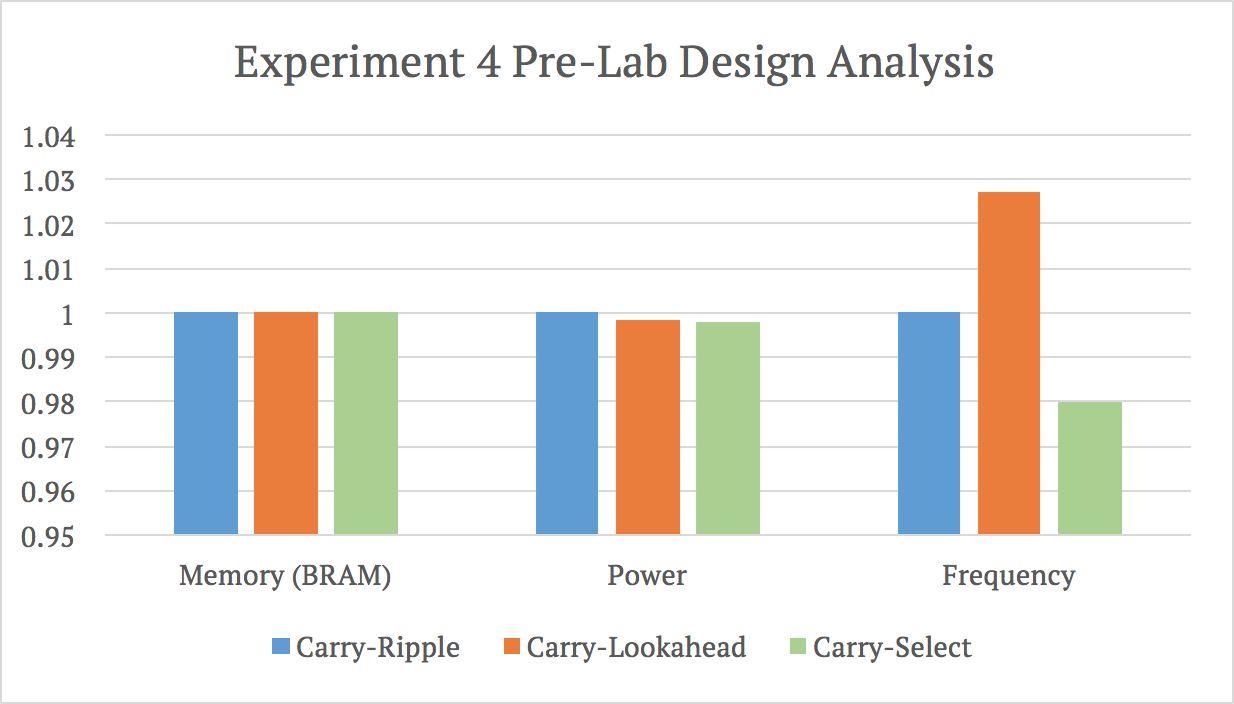
\includegraphics[scale=0.35]{pre-lab-design-analysis.png}
	\caption{Area, Power, Frequency Comparison\label{fig:pre-lab-design-analysis}}
\end{figure}


%SECTION 9 - Post Lab - Eric
\section{Post-Lab}
1) Compare the usage of LUT, Memory, and Flip-Flop of your bit-serial logic processor
exercise in the IQT with your TTL design in Lab 3. Make an educated guess of the usage of
these resources for TTL assuming the processor is extended to 8-bit. Which design is better, and
why? \\

Answer: The System Verilog design used in Lab 4 clearly dominates the total usage of Logic Elements in Lab 3 almost by a factor of three. This is because \_\_\_\_\_.
\begin{figure} [H]
	\centering
	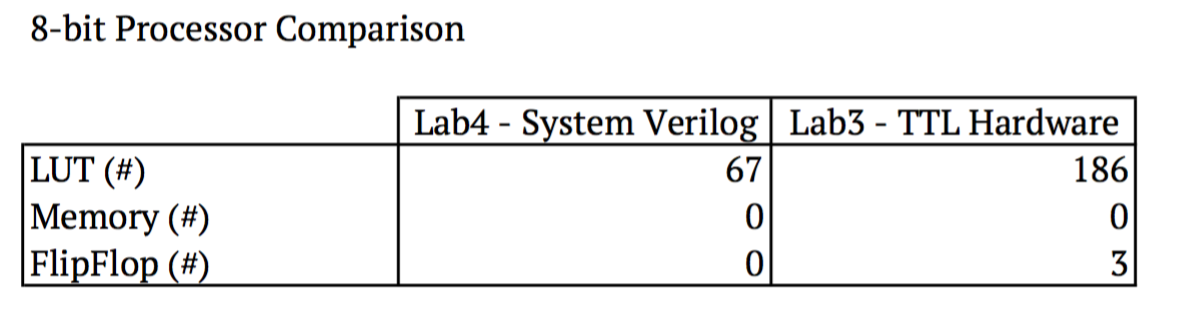
\includegraphics[scale=0.35]{processor-comparison.png}
	\caption{Processor Area Comparison\label{fig:processor-comparison}}
\end{figure}

2) For the adders, refer to the Design Resources and Statistics in IQT.30-32 and complete
the following design statistics table for each adder. This is more comprehensive than the above
design analysis and is required for every SystemVerilog circuit.

\begin{figure} [H]
	\centering
	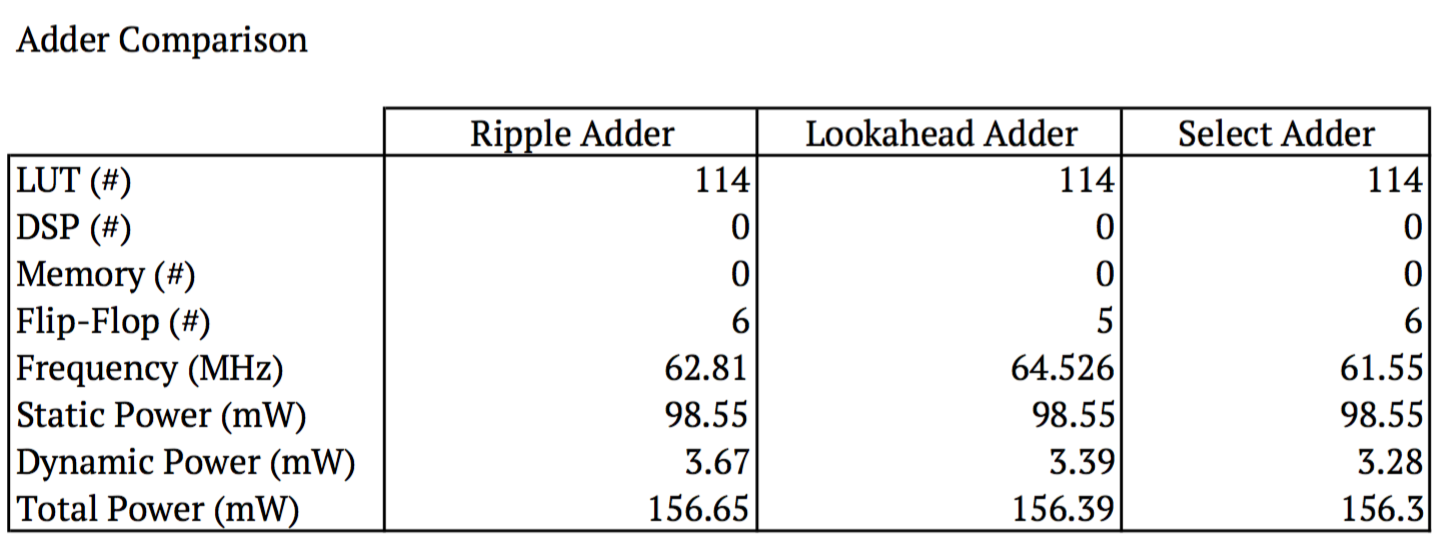
\includegraphics[scale=0.35]{lab4-statistics.png}
	\caption{Processor Area Comparison\label{fig:lab4-statistics}}
\end{figure}

%SECTION 10 - Conclusion - Eric
\section{Conclusion}
Overall, the team successfully demonstrated all three different adder designs for full credit. A

\hl{ERIC SECTION}


\clearpage
\onecolumn
%SECTION 11: Figures
\section{Figures}

\begin{figure} [htbp]
	\centering
	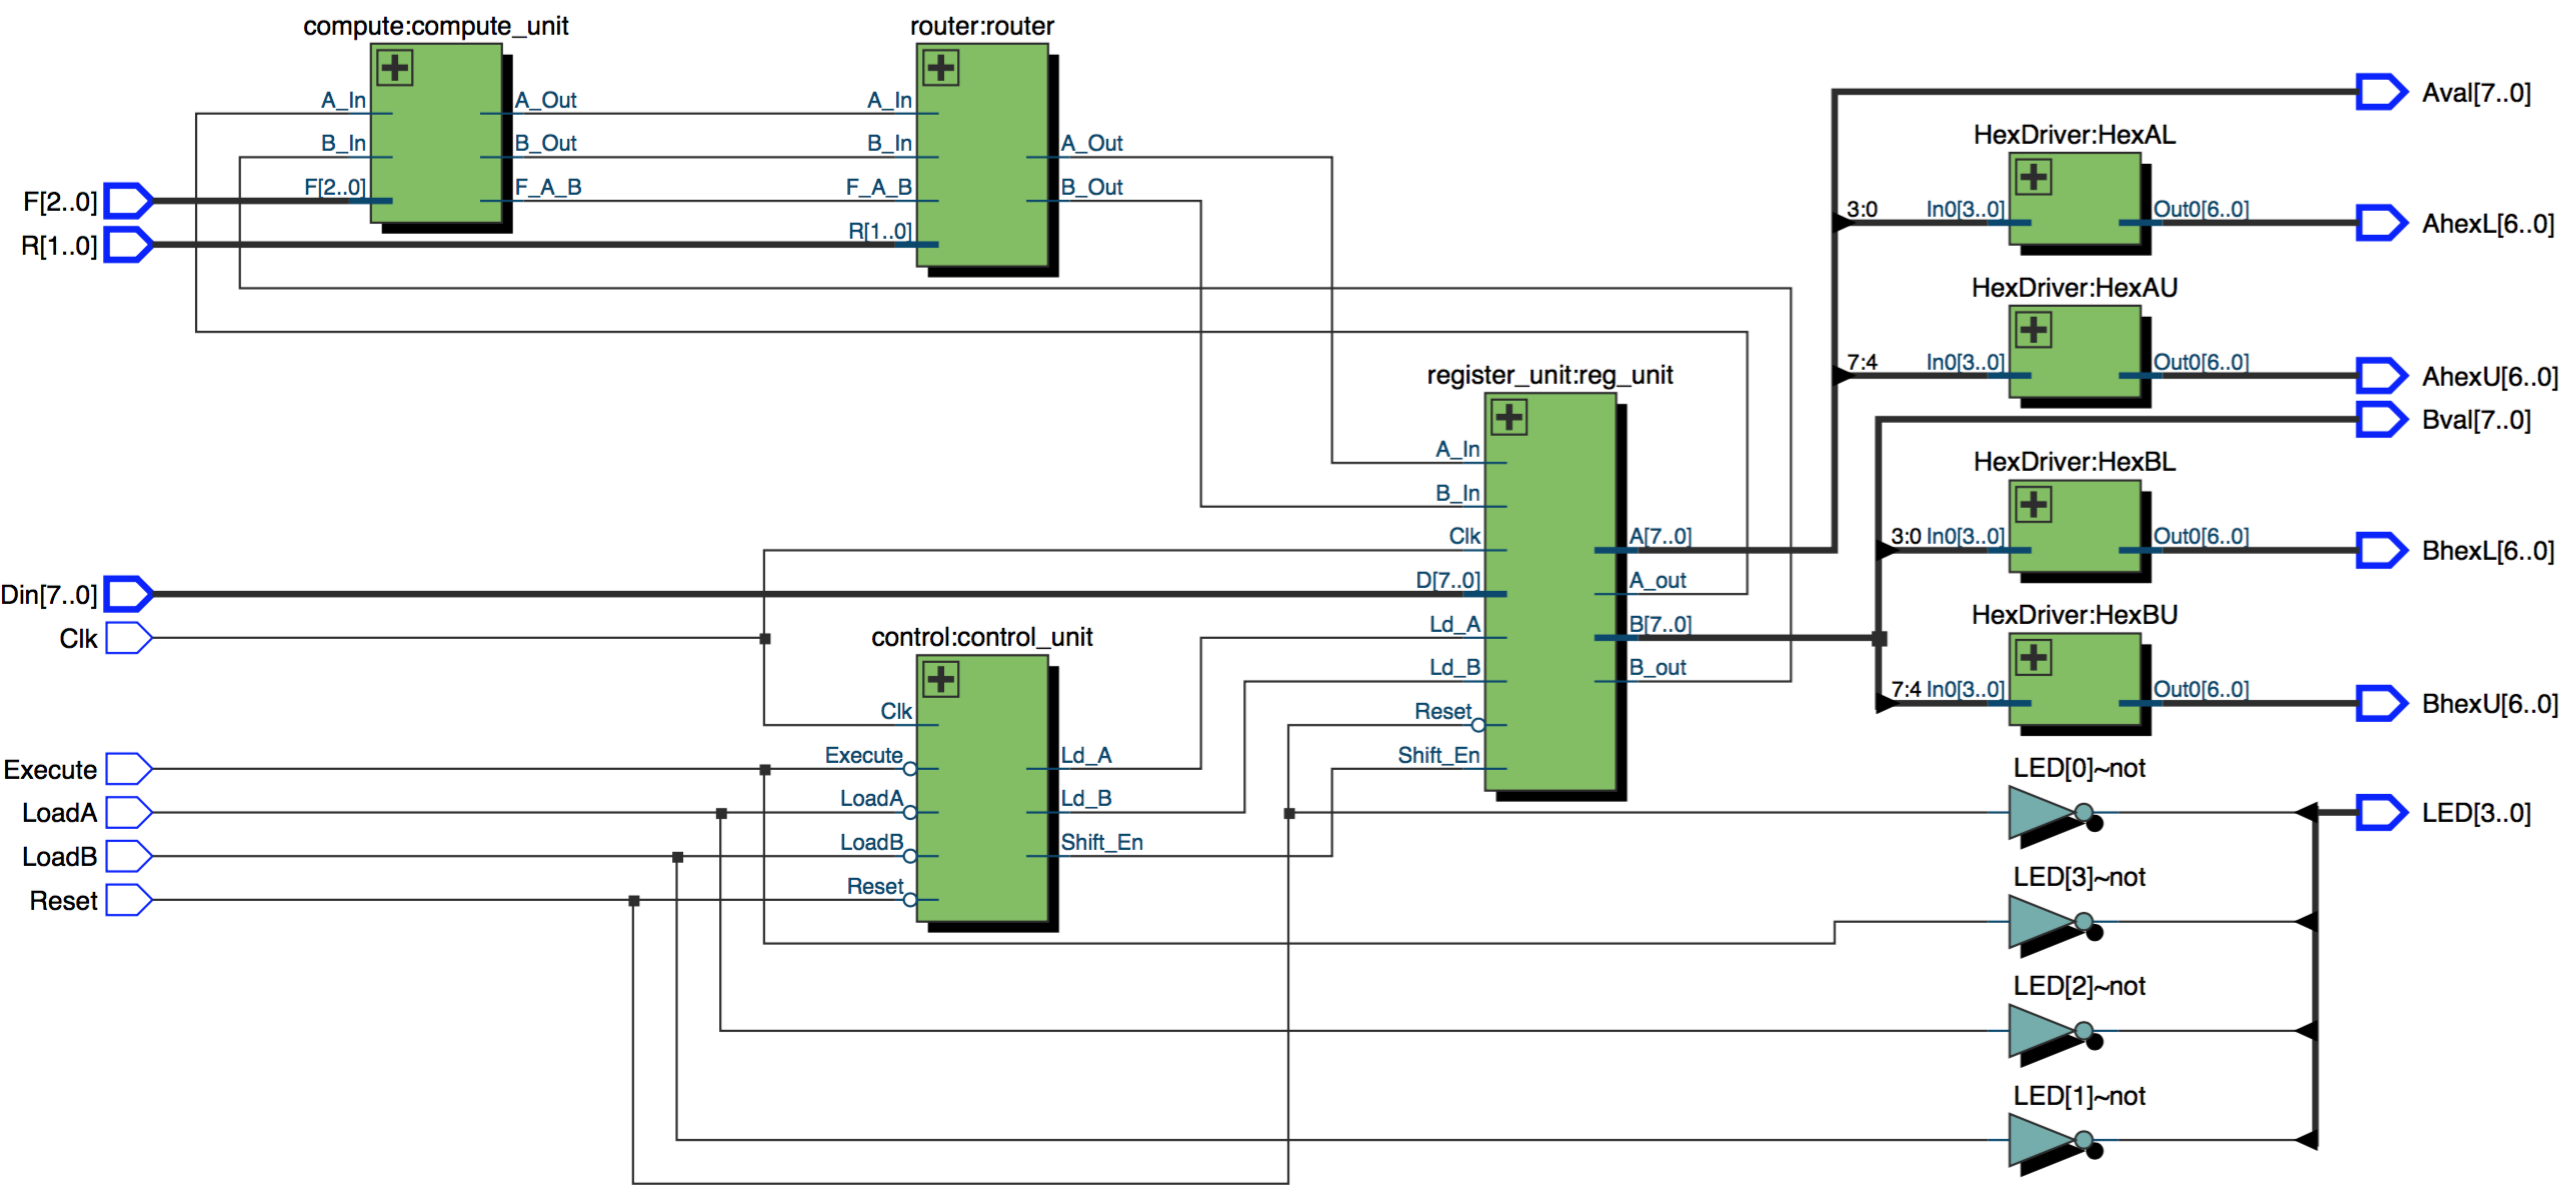
\includegraphics[scale=0.35]{Schematic-Processor.png}
	\caption{Serial Logic Processor Schematic\label{fig:schematic-processor}}
\end{figure}

\begin{figure} [htbp]
	\centering
	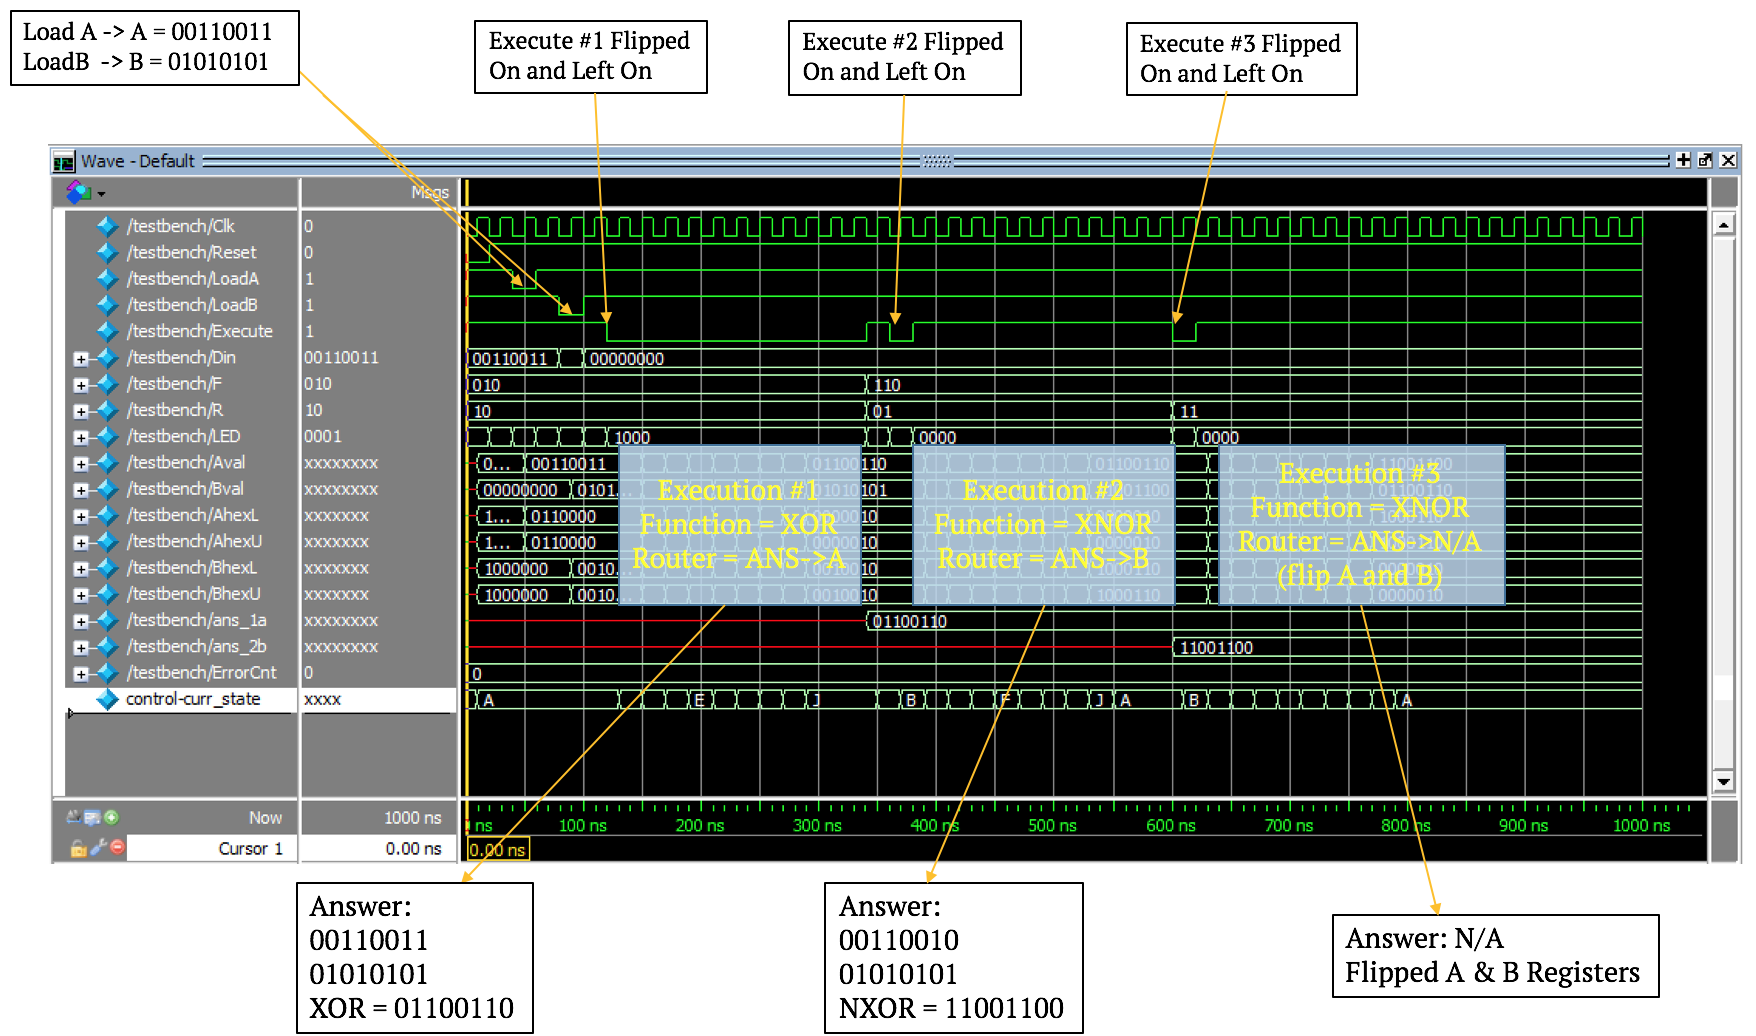
\includegraphics[scale=0.55]{processor-output-rtl-simulator.png}
	\caption{Serial Logic Processor RTL Simulation Output\label{fig:processor-output-rtl-simulator}}
\end{figure}

\begin{figure} [htbp]
	\centering
	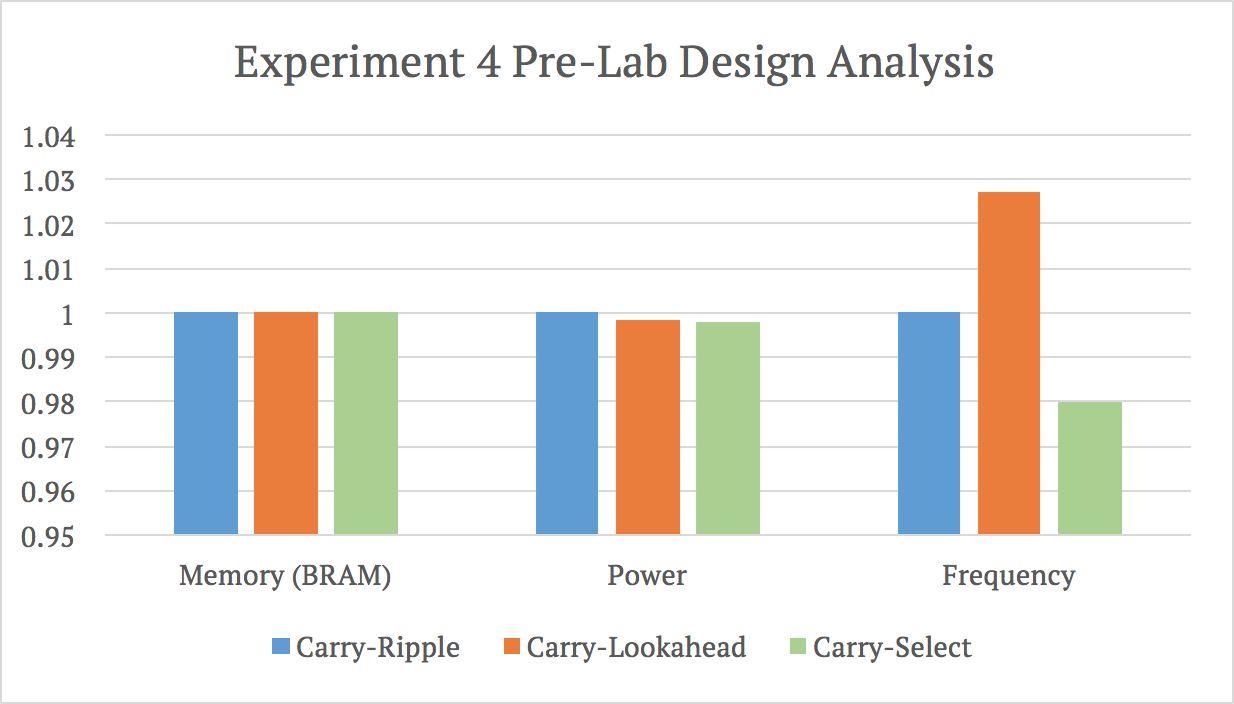
\includegraphics[scale=0.55]{pre-lab-design-analysis.png}
	\caption{Pre-Lab Adder Design Analysis (Area, Power, Frequency)\label{fig:pre-lab-design-analysis}}
\end{figure}



%SECTION : Bibliography
%Insert Bibliography if needed

\end{document}